\section{Design of OpenDT: an operational ecosystem for datacenter digital twinning}\label{sec:design}

In this section, we synthesise a set of functional and non-functional requirements for OpenDT, a digital twinning ecosystem for ICT infrastructure.

\subsection{Use Case Analysis}\label{sec:design:usecases}

\begin{enumerate}[label=\textbf{(UC\arabic*)},leftmargin=0pt,itemindent=3em]
    \item \label{design:uc1} \textbf{Monitoring and operation datacenters}: The design should aid practitioners in monitoring the performance and sustainability datacenters. The design should aid practitioners conduct twin-aware and simulation-aware infrastructure steering decisions.
    \item \label{design:uc2} \textbf{Researching ICT infrastructure} The systems should allow scientific researchers to conduct large-scale experiments and what-if analysis in a time and cost efficient way, while still maintaining accuracy and precision of the simulation results.
    \item \label{design:uc3} \textbf{Education} The system should serve (also) as educational material and aid in teaching computer systems courses, thus helping in educating future generations of responsible computer scientists and engineerings.
\end{enumerate}

\subsection{Requirement Analysis}\label{sec:design:requirements}

\begin{enumerate}[label=\textbf{(FR\arabic*)},leftmargin=0pt,itemindent=3em]
    \item \label{design:fr1} \textbf{Digital twin physical ICT infrastructure}: The ecosystem should digitally reflect physical datacenters, through a digital twin, continuously updated based on continuously ingested telemetry data. 
    \item \label{design:fr2} \textbf{Simulate with state-of-the-art scientific instrument}: The digital twinning ecosystem should adopt a peer-reviewed datacenter simulator with capabilities of predicting the performance, energy consumption, and CO2 emissions of infrastructure under workload.
    \item \label{design:fr3} \textbf{Suggest SLO-aligned changes of the physical twin}: The digital twinning ecosystem should suggest SLO-oriented adjustments of the physical twin, through topology adjustments based on machine learning, and further validated and compared through simulation. The ecosystem should select the topology best aligned with SLOs, based on simulation predictions.
    \item \label{design:fr4} \textbf{Autonomous, human-in-the-loop validated}: The ecosystem should be fully autonomous, with the physical twin continuously communicating with the digital twin (and vice-versa) at an operator-established granularity. The ecosystem should allow a human-in-the-loop for optional feedback validation.

    % modularity
\end{enumerate}

\begin{enumerate}[label=\textbf{(NFR\arabic*)},leftmargin=0pt,itemindent=3em]
    \item \label{design:nfr1} \textbf{Rapid, efficient digital twinning}: The digital twin component of the ecosystem receives monitoring data (telemetry) at operator-established granularity; the community standard of datacenter monitoring is 300 seconds~\cite{DBLP:conf/ccgrid/MastenbroekAJLB21, nicolae5377101m3sa, DBLP:journals/fgcs/MastenbroekMBI25}. 
    The digital twin should provide adjustment feedback within 300 seconds, while still meeting the other requirements and not distrubing the operation of the physical twin.
    % ($T_d$), while still adhering to the other requirements, within the monitoring timeframe ($\Delta T_{m}$) minus the time needed for the physical infrastructure to adapt ($T_{i}$): $T_d = T_m - T_i$. For example, for a monitoring granularity of 300 seconds, and a physical infrastructure adjustment of 30 seconds, the digital twinning ecosystem should provide feedback within 270 seconds.
    
    \item \label{design:nfr2} \textbf{Accurate adjustment feedback}: The ecosystem should include a machine-learning algorithm for adjusting topologies towards meeting operator-established SLOs. The topologies should be evaluated by simulation, and the overall-best topology meets SLOs in 100\% of the time. 
    
    \item \label{design:nfr3} \textbf{Massive-scale operation}: The ecosystem should support operation at scale, support telemetry and input traces from real-world datacenters (e.g., SURF), spanning over days of operation, and operate while still meeting the other established requirements.
\end{enumerate}



\subsection{Overview of the OpenDT Design and Operation Model}\label{sec:design:choices}
\Cref{fig:opendt-design} depicts a high-level overview of OpenDT. We design OpenDT as a modular digital twinning ecosystem for operating and monitoring datacenters \ref{design:fr1}, either autonomously or following the human-in-the-loop paradigm (HITL) \ref{design:fr4}. In this work, we adopt OpenDC, a peer-reviewed, open-source, discrete-event simulator, with over 7 years of development and operation~\cite{DBLP:conf/ccgrid/MastenbroekAJLB21, DBLP:journals/fgcs/MastenbroekMBI25, nicolae5377101m3sa}.

\textit{Orchestrator:} OpenDT adopts a central orchestration component~\circled{A} for 1) handling communication between the physical and digital twin~\circled{C}-\circled{I}, 2) managing human input and displaying ecosystem output, via a dashboard~\circled{E}, and 3) storing ecosystem snapshots in a datalake~\circled{G}.

\textit{Physical:} The physical twin~\circled{C} (physical datacenter) is monitored by a telemetry system~\circled{B}, which transfers data to the orchestrator. The adjuster~\circled{D} receives data from the orchestrator and goal-oriented steers the infrastructure.

\textit{Digital:} The digital twin~\circled{I} (virtual copy of the physical datacenter) is continuously updated with real-world information, at a user-established granularity, by a handler~\circled{H}. The handler, serves as an adjuster with extended capabilities: 1) adjusts the digital twin to reflect the measured reality, 2) conducts what-if analysis, where topology changes are proposed by a an LLM, SLO-aware system, validated through simulation, and tailored to meet SLOs, and 3) communicates to the orchestrator the topology adjustment best aligned with SLOs.

\textit{The human in the loop:} OpenDT adopts a human-in-the-loop (HITL) operational paradigm, where the digital twinning ecosystem operates autonomously, yet the human can (optionally) intervene and dictate decision-making processes. The human operator~\circled{F} reads data and controls the ecosystem via a dashboard~\circled{E}. We identify two main design choices of autonomous operation: (DC1) where the ecosystem operates isolated from external input, and only SLOs dictate, and (DC2) where the ecosystem operates aligned with SLOs, yet with a HITL who can accept, adjust, or reject the ecosystem's decisions. According to the keynote on Digital Twins of datacenters, from Alexandru Iosup, at ModSim 2024, Brookhaven National Laboratory, on \textit{``A VU on Digital Twins to Improve the Performance and Technological Sustainability of Data Centers in the
Continuum,"} ~\cite{ModSim2024Agenda} (DC2), unlike (DC1), which omits a HITL, is ethically viable for operating datacenters running (also) critical workload tasks where the twinning ecosystem could prioritise meeting SLOs over human or security well-being. One such unethical decision could be the ecosystem prioritising a batch of tasks from industry, which pays better, instead of a critical batch of tasks from a hospital, whose patients' lives can depend on. Therefore, although theoretically such scenarios can be prevented by perfectly-established SLOs and perfectly-engineered digital twinning ecosystems, in reality, perfection is unachievable in distributed, massive-scale computer ecosystems and even small operational errors could cause critical disruptions~\cite{Iosup2024DigitalTwins}.

\textit{Every-window process:} We envision OpenDT as twinning at a user-established granularity, making the digital twin also compatible with a discrete-event simulator; the industry-standards sampling rate in datacenters is 300 seconds~\cite{DBLP:conf/ccgrid/MastenbroekAJLB21, DBLP:journals/fgcs/MastenbroekMBI25}, yet we regard a practitioner-adjustable granularity as best suited for our design. OpenDT operates in fixed windows of 300 seconds, thus handling events regularly, able to replay historical situations and conduct discrete-event simulation. At each window start, OpenDT ingests telemetry~\circled{B}, updates the digital representation of the physical twin (i.e., the digital twin, component~\circled{I}), simulates with OpenDC~\circled{J}, checks SLOs~\circled{H}, and proposes validated topology deltas~\circled{H}. Then, OpenDC displays the snapshot and the deltas on the dashboard~\circled{A}, awaiting HITL approval for major decisions~\circled{F}, or proceeds without such approval for minor decisions. Lastly, decisions are forwarded to an actuator, the PT Adjuster \circled{D}, and also written, immutably, in the data lake~\circled{G}. 

\textit{OpenDT's time snapshot:} OpenDT's time snapshot at time~$t$ contains four (three plus one) main components: 1) topology and fragments yet to be executed at $t$, 2) the energy consumption (watt-hours) at $t$, 3) the CO2 emissions at $t$ (gCO2), although not used in the implemented prototype, still present for future work, 4) and the CPU usage per host (\%). Snapshots are received as telemetry data from the Physical Twin (in our prototype, from the virtual-physical-twin, Kafka-powered), and are immutable, at constant granularity (i.e., regular), and measured by sensors from the ICT infrastructure (specifically, which and what type of sensors, is dependent on the datacenter at subject).


%  \subsection{Human in the loop}
% OpenDT deploys a semi-autonomous system by having a human in the loop \circled{F} that reads the dashboard \circled{E} and either accepts or rejects the newest topology change proposed by the digital twin. The dashboard will present alongside the new recommended topology change, the state used by the digital twin to recommend this topology, and the current state of the physical twin (more details in implementation section), which are fetched from the data lake \circled{G} and the physical twin, respectively. In the future versions of OpenDT we strive to make this control loop fully autonomous, but since we don't have a real data center to use as a physical twin and the low maturity level of our current version of OpenDT, we leave full autonomy for later.



% We analyze two design choices of the interaction between components \circled{H}, \circled{J}, and \circled{I}, which ensures SLO-aligned changes and feedback \ref{design:fr3}. We first identify a design choice where the handler both controls the simulator and directs topology-specific data to the simulator. We also identify a design choice the simulator receives control from the handler and exract datacenter topology from the digital twin component~\circled{I}. We regard the latter as better aligned with \ref{design:nfr3}, potentially allowing parallelisation, and, thus, better scalability when the digital twinning ecosystem would operate at scale.

% We adopt OpenDC simulator~\circled{H} to predict performance and sustainability of various topologies. We also adopt reinforcement-learning (RL) in component~\circled{J}, where the digital twin handler would use RL for predicting the best topology adjustment such that SLOs are best met. These topologies are validated by the simulator (\circled{H}) for at most the amount of time between two sampling intervals, and, when the time is up, the handler~\circled{J} selects and forwards the overall best topology feedback to the orchestrator. 

% The orchestrator appends the snapshot into a datalake~\circled{G}, and displays to a HITL on an interactive dashboard~\circled{E}. The orchestrator forwards the HITL's feedback to a physical twin adjuster~\circled{D}, which adapts the physical twin (i.e., datacenter) accordingly.


% OpenDT contains a central orchestrator component~\circled{A}, which handles the communication between the physical~\circled{C} and the digital twin~\circled{I}, as well as reflecting information to a monitoring and control dashboard~\circled{E}. 

% In the physical component, the physical twin \circled{C} is measured by a telemetry system~\circled{B}, which sends telemetry data to the orchestrator~\circled{A}. The orchestrator stores telemetry in a data lake~\circled{G}, and displays relevant information on a dashboard~\circled{E}, the main interaction point of the human-in-the-loop. Then, the orchestrator updates the digital twin via a handler component \circled{J}.


\subsection{OpenDC simulator as a representation model }\label{sec:design:simulation-models}
{
\SetTblrInner{colsep=1.25pt}
\renewcommand{\arraystretch}{0.94}
\begingroup
% keep math inline on one line (no wrapping in X)
\everymath{\displaystyle}%
\begin{table}[t]
\centering
\begin{tblr}{
% narrow Name, flexible Formula, narrow Source
colspec = {Q[l,wd=1.1cm] X Q[l,wd=1.8cm]},
width = \linewidth,
hline{1-2,9-10} = {-}{},
% avoid extra padding around cells
column{1,3} = {leftsep=0pt,rightsep=0pt},
column{2} = {leftsep=0pt,rightsep=0pt},
}
Name                 & Formula                                                                                                                             & ~Source \\ 
Sqrt                 & $P(u)=P_{\text{idle}}+(P_{\text{max}}-P_{\text{idle}})\sqrt{u}$ \label{eq:sqrt_power}                                              & \cite{DBLP:conf/iccS/SilvaOCTDS19, DBLP:journals/spe/CalheirosRBRB11, DBLP:conf/ccgrid/MastenbroekAJLB21} \\ 
Linear               & $P(u)=P_{\text{idle}}+(P_{\text{max}}-P_{\text{idle}})\,u$ \label{eq:linear_power}                                                 & \cite{DBLP:conf/iccS/SilvaOCTDS19, DBLP:journals/spe/CalheirosRBRB11, DBLP:conf/ccgrid/MastenbroekAJLB21} \\ 
Square               & $P(u)=P_{\text{idle}}+(P_{\text{max}}-P_{\text{idle}})\,u^{2}$ \label{eq:square_power}                                             & \cite{DBLP:conf/iccS/SilvaOCTDS19, DBLP:journals/spe/CalheirosRBRB11, DBLP:conf/ccgrid/MastenbroekAJLB21} \\ 
Cubic                & $P(u)=P_{\text{idle}}+(P_{\text{max}}-P_{\text{idle}})\,u^{3}$ \label{eq:cubic_power}                                              & \cite{DBLP:conf/iccS/SilvaOCTDS19, DBLP:journals/spe/CalheirosRBRB11, DBLP:conf/ccgrid/MastenbroekAJLB21} \\ 
MSE                  & $P(u)=P_{\text{idle}}+(P_{\text{max}}-P_{\text{idle}})\,(2u-u^{r})$ \label{eq:mse_power}                                           & \cite{DBLP:conf/ccgrid/MastenbroekAJLB21, DBLP:conf/isca/FanWB07} \\ 
Asym           & $P(u)=P_{\text{idle}}+\dfrac{P_{\text{max}}-P_{\text{idle}}}{2}\bigl(1+u-e^{-u/\alpha}\bigr)$ \label{eq:asymptotic_power}          & \cite{DBLP:conf/ccgrid/MastenbroekAJLB21} \\ 
AsymD      & $P(u)=P_{\text{idle}}+\dfrac{P_{\text{max}}-P_{\text{idle}}}{2}\bigl(1+u^{3}-e^{-u^{3}/\alpha}\bigr)$ \label{eq:asymptotic_power_dvfs} & \cite{DBLP:conf/ccgrid/MastenbroekAJLB21} \\ 
\end{tblr}
\vspace{0.3cm}
\caption{Formulas of the power models OpenDC uses to predict energy usage. $P_{\text{idle}}$, $P_{\text{max}}$ are the powers in idle and full-capacity states, $u$ is device utilization, $e$ is Euler’s number, $\alpha$ is the utilization fraction at which the host becomes asymptotic, and $r$ is a calibration parameter. Table adapted from~\cite{nicolae5377101m3sa}.}
\label{table:power-draw-formulas}
\end{table}

We use OpenDC as a the representation model of the system and, overall, of the environment~\cite{DBLP:conf/ccgrid/MastenbroekAJLB21}. OpenDC is a peer-reviewed, open-source, discrete-event simulator with simple interfaces, and over 8 years of development and operation~\cite{nicolae5377101m3sa}. OpenDC supports what-if analysis of datacenter infrastructure, simulation driven, in a time and cost-efficient way, and provides various features such as simulation of workloads of various natures (e.g., scientific jobs, business-critical), multi-model and meta-model simulation~\cite{nicolae5377101m3sa}, serverless processes, operational phenomena-aware simulation (i.e., infrastructure failures), or tensorflow simulation. Although, for the current version of OpenDT we do not employ complex simulation techniques (e.g., meta-model simulation), we regard as crucial for future development of OpenDT to employ a simulation instrument capable of advanced, complex, high-fidelity simulation.

In this work, especially in the prototyping component, we only consider the power draw due to CPU usage. 
However, OpenDT coupled with OpenDC supports modelling the power draw, and thus energy consumption, of various hardware components. \Cref{table:power-draw-formulas} shows the power models OpenDT inherits from the peer-reviewed OpenDC~\cite{DBLP:conf/ccgrid/MastenbroekAJLB21}; In this work, we utilize linear power models, yet configure the ecosystem as capable of predicting using (and including) latest state-of-the-art simulation techniques in the community, such as multi-model and meta-model simulation~\cite{nicolae5377101m3sa}.



\subsection{LLM-based datacenter monitoring and steering}\label{sec:design:llm}

\begin{lstlisting}[style=pyopendt,
  caption={OpenDT LLM prompt to request SLO-aligned topology changes.},
  label={lst:opendt-prompt},
  captionpos=b, % put caption below
  float=!htbp  % let it float like figures
]
"""You are an expert datacenter practitioner. 
Based on these simulation results, provide specific recommendations to optimize energy utilization and performance (execution time).

You will be provided data from OpenDC simulator which simulates datacenter energy usage and runtime.
You need to recommend next core count and core speed for simulation for each cluster and host.

You need to recommend similar configuration which helps to achieve objectives:
- Lesser runtime
- Less energy consumption

Try to achieve both objectives(SLOs) at the same time as much as possible:
{slo_targets}

SIMULATION RESULTS:
- Energy Usage: {sim_results.get('energy_kwh', 'N/A')} kWh
- Runtime: {sim_results.get('runtime_hours', 'N/A')} hours
- CPU Utilization: {sim_results.get('cpu_utilization', 'N/A')}
- Task Count: {batch_data.get('task_count', 'N/A')}  
- Fragment Count: {batch_data.get('fragment_count', 'N/A')}
- Average CPU Usage: {batch_data.get('avg_cpu_usage', 'N/A')}

Current topology: {json.dumps(current_topology, indent=2) if current_topology else 'Not provided'}

{parser.get_format_instructions()}

Example:
{{
"cluster_name": ["C01", "C01"],
"host_name": ["H01", "H02"],
"coreCount": [32, 16],
"coreSpeed": [3200, 2100],
"count": [2, 3]
}}
"""
\end{lstlisting}

In this work, we employ OpenAI’s GPT-3.5 Turbo, a large language model (LLM) capable of both conversational and traditional text-generation tasks, to develop a Topology Recommendation System~\citationsneeded{1}. 
GPT-3.5 Turbo demonstrates strong capabilities in natural language understanding and code generation~\citationsneeded{2}, making it applicable across diverse domains such as dialogue systems, code synthesis, and content generation. 
In OpenDT, we use GPT-3.5 to generate topological configurations for datacenter simulations and ensure the infrastructure remains aligned with SLOs, as workloads change; 
for example, although more tasks may arrive, the LLM should ensure an SLO-compliant execution time and resource utilization.



The LLM is guided through prompt engineering, wherein contextual information is provided, including the results of OpenDC simulations for the current topology, and the corresponding Service Level Objectives (SLOs). 
Based on this input, the model infers and recommends new topological parameters—such as the number of hosts, clock speed, and number of cores—that are expected to yield improved performance.
We present in \Cref{lst:opendt-prompt} the prompt OpenDT uses to adjust ICT configuration and aim to meet the SLOs. The prompt follows community-established principles of prompt engineering~\citationsneeded{2}, and is structured in four main components: 1) the LLM receives a role, specifically \textit{``datacenter practitioner"}, 2) the LLM receives the task, specifically to adjust the topology such that SLOs are met, 3) the LLM receives the user-(practitioner-)defined SLOs and the topology at the given timestamp, and, lastly, 4) the LLM receives the output format. To prevent errors, OpenDT validates and further processes prompts only if the LLM's (non-deterministic) output matches the format requested in the prompt.


\begin{figure}[t]
    \centering
    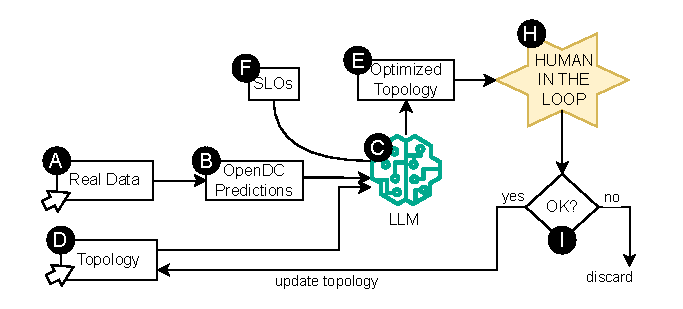
\includegraphics[width=\linewidth]{report/figures/llm-hl-overview.pdf}
    \caption{Overview of the LLM-based topology recommendation system OpenDT adopts. Overall, OpenDT is designed as modular and is able to select any API-callable LLM, through minor codebase modifications.}
    \label{fig:llm-overview}
\end{figure}

Furthermore, in \Cref{fig:llm-overview}, we present a high-level overview of the proposed topology recommendation system. The process begins when a real-time data stream \circled{A} is fed into OpenDC, which performs the simulation and produces the baseline results \circled{B}. These results, together with the current topology \circled{D} and the system’s SLOs \circled{F}, are then provided as contextual input to the LLM \circled{C}. Then, the LLM analyzes this information and predicts an optimized topology configuration that is expected to yield improved simulation results. The newly recommended topology is subsequently fed back into OpenDC \circled{E} to generate optimized simulation results. Finally, a human decision-maker \circled{H} evaluates these results and decides whether to accept or reject the recommendations generated by LLM \circled{I}. If the new, optimized topology, is accepted, component topology \circled{D} is updated.
